\documentclass{article} 

%----------------------------------------    
%------------------------------------------------------------------- 
    \usepackage[utf8]{inputenc} %just do it
    \usepackage[english]{babel}
    \usepackage{graphicx} %allows images
        \graphicspath{documents/}
    \usepackage{amsmath} %allows maths equations
    \usepackage{geometry} %allows editing of page geometry (https://www.overleaf.com/learn/latex/Page_size_and_margins)
        \geometry{
            a4paper,
            top=0.7in,
            bottom=1in,
            textwidth=7in
            }
    \usepackage{sectsty} %alter section title formatting
        \sectionfont{\fontsize{13}{16}\selectfont}
    \usepackage{tabularx}
    \usepackage[table]{xcolor}
    \usepackage{enumitem}
    \usepackage{color, colortbl}
    \usepackage{tikz}                   
    \usetikzlibrary{shadows}
    \usepackage{transparent}
    \usepackage[framemethod=tikz]{mdframed}
    \usepackage{lipsum}
    \usepackage{tikz,lipsum,lmodern}
    \usepackage[most]{tcolorbox}
    \usepackage{tikz}
    \usepackage{tabularx}
    \usepackage{hyperref}
        \hypersetup{
        colorlinks=true,
        linkcolor=blue,
        filecolor=magenta,      
        urlcolor=cyan,
        }
%-------------------------------------------------------------------         %----------------------------------------    



    \title{\textbf{WTTS}}
    \author{Rahul Kakaiya}
    \date{}
    
    \newcommand\customfont[1]{\usefont{'playtime.ttf'}}
    
    \renewcommand{\arraystretch}{3}
    
    \definecolor{purple}{RGB}{142, 68, 173}
    \definecolor{blue}{RGB}{52, 152, 219}
    \definecolor{orange}{RGB}{243, 156, 18 }
    \definecolor{red}{RGB}{231, 76, 60}
    \definecolor{turquoise}{RGB}{26, 188, 156}
    \definecolor{dblue}{RGB}{31, 97, 141}
    \definecolor{lblue}{RGB}{21, 204, 236}
    \definecolor{dgreen}{RGB}{22, 137, 45}
    \definecolor{green}{RGB}{0, 184, 47}
    
    \newcommand\invisiblesection[1]{
    \refstepcounter{section}
    \addcontentsline{toc}{section}{\protect\numberline{\thesection}#1}
    \sectionmark{#1}}
    
    \newcommand\invisiblesubsection[1]{
    \refstepcounter{subsection}
    \addcontentsline{toc}{subsection}{\protect\numberline{\thesubsection}#1}
    \sectionmark{#1}}
    
    \newenvironment{white}{\color{white}}{\ignorespacesafterend}
    
    
    
%----------------------------------------
%-------------------------------------------------------------------





\begin{document}

    \begin{table}[h!]
    \begin{centering}
    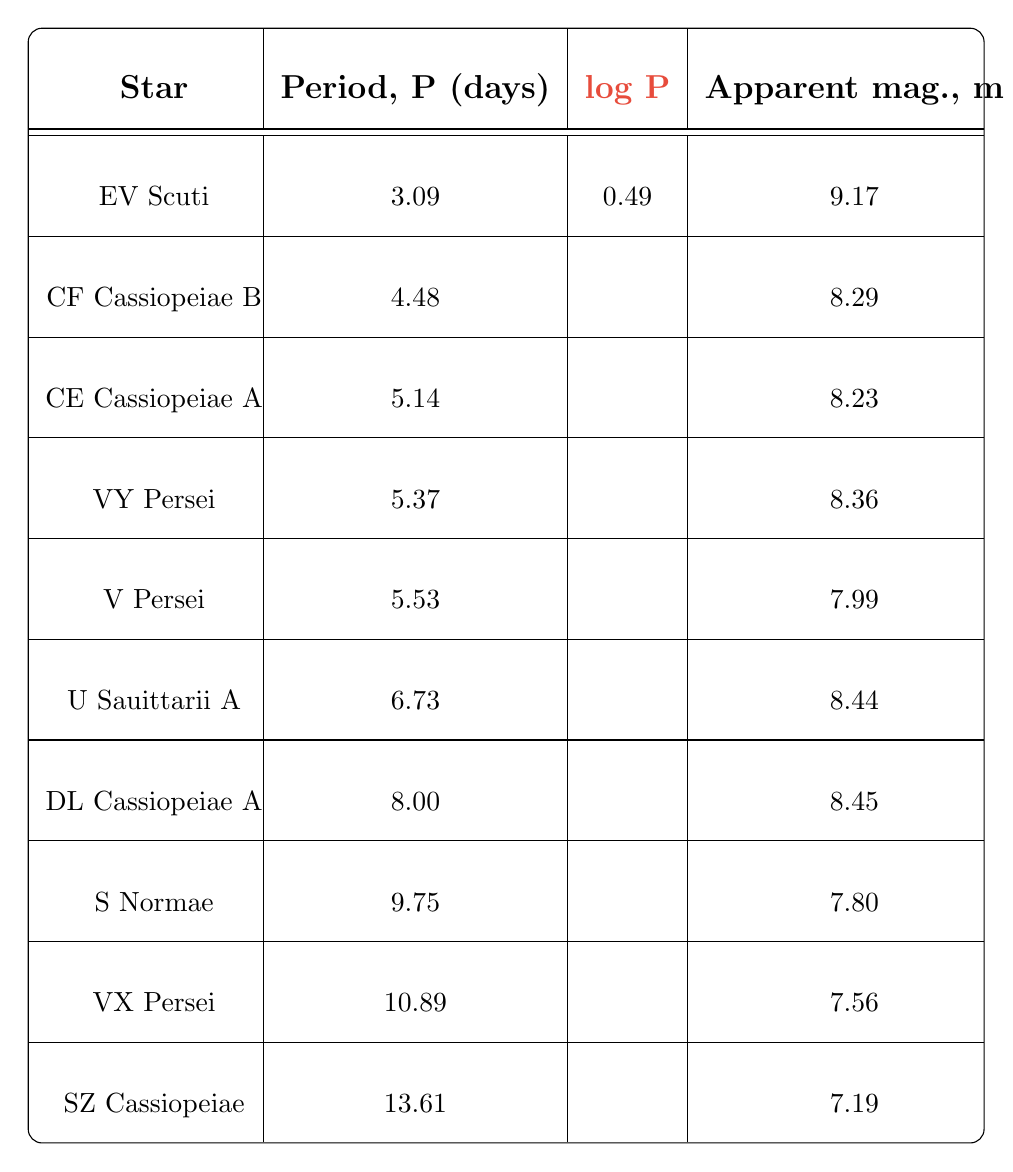
\begin{tikzpicture}
    \node (table) [inner sep=0pt] {
    \begin{tabular*}{\textwidth}{c @{\extracolsep{\fill}} |c|c|c|cc }
        \large\textbf{\textcolor{black}{Star}} & \large\textbf{\textcolor{black}{Period, P (days)}} & \large\textbf{\textcolor{red}{log P}} & \large\textbf{\textcolor{black}{Apparent mag., m}} & \large\textbf{\textcolor{red}{Absolute mag., M}}\\
        \hline\hline
        EV Scuti & 3.09 & 0.49 & 9.17 & -2.90  \\
        \hline
        CF Cassiopeiae B & 4.48 &  & 8.29 &  \\
        \hline
        CE Cassiopeiae A & 5.14 &  & 8.23 &  \\
        \hline
        VY Persei & 5.37 &  & 8.36 &  \\
        \hline
        V Persei & 5.53 &  & 7.99 &  \\
        \hline
        U Sauittarii A & 6.73 &  & 8.44 &  \\
        \hline
        DL Cassiopeiae A & 8.00 &  & 8.45 &  \\
        \hline
        S Normae & 9.75 &  & 7.80 &  \\
        \hline
        VX Persei & 10.89 &  & 7.56 &  \\
        \hline
        SZ Cassiopeiae & 13.61 &  & 7.19 & \\
    \end{tabular*}
    };
    \draw [rounded corners=.5em] (table.north west) rectangle (table.south east);
    \end{tikzpicture}
    \end{centering}
    \caption{\label{tab:table-name}Data about a range of Cepheid variable stars in the Galaxy.}
    \end{table}

\newpage

    \begin{figure}[h]
        \caption{Light diagram for Cepheid variable star located in the Pearl cluster}
        \centering
        \includegraphics[width=1\textwidth]{cepheid-light-diagram.png}
    \end{figure}
    
\newpage
    
    
%%%%%%%%%%%%%%%%%%%%%%%%%%%%%%%%%%%%%%%%%%%%%%%%%%%%%%%  

    \begin{enumerate}[label=\color{dblue}\theenumi]
        \item In this activity you will be finding the distance to the Pearl Star Cluster, containing the C1 Pinnea Cepheid variable star.
        \begin{itemize}
            \item By using Henrietta Swan Leavitt's \emph{\textcolor{orange}{period-luminosity relationship}}, you will find the distance to the nearby Cepheid variable star and therefore the distance to the star cluster that it is in.
            \item You will be introduced to the computer programming language \emph{\textcolor{orange}{'Python'}} and will use a piece of code as a tool to interpolate the period-luminosity graph for the C1 Pinnea Cepheid variable star.
            \item In order to measure the distance to a new star cluster we must find the absolute magnitude, \textbf{\textcolor{red}{\(M\)}}, of the Cepheid variable star inside of the cluster.\\
        \end{itemize}
    \end{enumerate}

    %task 1
    \begin{tcolorbox}[enhanced,attach boxed title to top center={yshift=-3mm,yshifttext=-1mm},colback=dblue!90!white,colframe=dblue!80!white,colbacktitle=dblue!80!black,title=Activity 1 - Distance Determination,fonttitle=\bfseries,boxed title style={size=small,colframe=dblue!80!black}]
        \begin{bfseries}
        \begin{white}
            \begin{enumerate}
                
                \item Using the your calculator and the distance modulus relationship equation, calculate and complete the missing data of Cepheid variable stars in the Galaxy in table 1.
                
                \item Open the website: \href{https://repl.it/languages/python3}{\texttt{https://repl.it/languages/python3}}. Copy and paste the code from the file '\texttt{distance-determination.py}' to the left hand side of the website interface. 
                
                \item This code will create a period-luminosity relationship for the Cepheid variable stars in table 1. From the table, which variable would be on which axis for this graph? Once you've decided, label each axis in the code: (\texttt{\textcolor{green}{plt.xlabel('}\textbf{\textcolor{red}{x-label}}\textcolor{green}{')}}) (\texttt{\textcolor{green}{plt.ylabel(}'\textbf{\textcolor{red}{y-label}}\textcolor{green}{')}}). Check with your teacher before moving on to the next step.
                
                \item Using the data you have calculated in table 1, input the \(x\) and \(y\) axis data for the period-luminosity graph into the computer code. These values will be inputted here in the code: \texttt{\textcolor{green}{x = np.array([}\textbf{\textcolor{red}{data-point-1,data-point-2,etc}}\textcolor{green}{])}} for the \(x\) values, \texttt{\textcolor{green}{y = np.array([}\textbf{\textcolor{red}{data-point-1,data-point-2,etc}}\textcolor{green}{])}} for the \(y\) values. 
                
                \item Click \texttt{\textcolor{cyan}{run}} and allow the code to execute. A new image called \texttt{\textcolor{cyan}{cepheid.png}} will be created and display in the bottom right. Can you clearly see Henrietta Swan Leavitt's period-luminosity relationship? The gradient and y-intercept of this relationship is displayed in the top right. What is the equation of the line?
                
                \item Figure 1 shows the light diagram for C1 Pinnea Cepheid observed in the Pearl cluster. Estimate the oscillation period by reading x-axis minima/maxima periodicity.
                
                \item Using the period of C1 Pinnea and the equation of the line of the period-luminosity relationship, calculate C1 Pinnea's absolute magnitude, \textbf{\textcolor{green}{\(M\)}}. The average apparent magnitude, \textbf{\textcolor{green}{\(m\)}}, of C1 Pinnea is 15.26.
        
            \end{enumerate}
        \end{white}
        \end{bfseries}
    \end{tcolorbox}
% - plot the P-L graph in a python code -> analyse the graph to read the luminosity given the period -> use M m and P to find D

%%%%%%%%%%%%%%%%%%%%%%%%%%%%%%%%%%%%%%%%%%%%%%%%%%%%%%%   
    
    
    
\newpage
    
    
    
%%%%%%%%%%%%%%%%%%%%%%%%%%%%%%%%%%%%%%%%%%%%%%%%%%%%%%%%%

    \begin{enumerate}[label=\color{purple}\theenumi]
    \setcounter{enumi}{1}
        \item In this activity you will be finding the age of the Pearl star cluster by comparing observed data to simulated isochrones.
        \begin{itemize}
            \item By comparing observed HR data with stellar isochrones formed from simulated HR-diagrams for a population of stars, you will approximate the age of the Pearl star cluster.
            \item You will be introduced to the \emph{\textcolor{orange}{WTTS software}}. You will also continue working with \emph{\textcolor{orange}{'Python'}} code to automate data analysis processes.\\
            \item If you're interested in learning simple mathematical computer programming from the ground up, check out \href{https://projecteuler.net/}{https://projecteuler.net/} which has an archive of exercises mathematical computer programming exercises from beginner level all the way up.
            \item Another place to learn useful problem solving skills is \href{https://isaacphysics.org/alevel}{https://isaacphysics.org/alevel}. The skills that these two websites can help develop are critical in science and scientific research, and it is all available for free!
        \end{itemize}
    \end{enumerate}
    
    
    %task 2
    \begin{tcolorbox}[enhanced,attach boxed title to top center={yshift=-3mm,yshifttext=-1mm},colback=purple!90!white,colframe=purple!80!white,colbacktitle=purple!80!black,title=Research Project - The Red Giant Branch,fonttitle=\bfseries,boxed title style={size=small,colframe=purple!80!black}]
        \begin{bfseries}
        \begin{white}
            \begin{enumerate}
                \item Using the table above, you will use the stellar evolution software 'Window To The Stars' (WTTS) to evolve a range of theoretical stars and categorise them (do they evolve into red giants, red super-giants, blue giants or white dwarfs?). \emph{Open 'WTTS Basic'}.
            \end{enumerate}
        \end{white}
        \end{bfseries}
    \end{tcolorbox}
    
%%%%%%%%%%%%%%%%%%%%%%%%%%%%%%%%%%%%%%%%%%%%%%%%%%%%%%%%    



\newpage



%-----4. ISOCHRONES-----
%%%%%%%%%%%%%%%%%%%%%%%%%%%%%%%%%%%%%%%%%%%%%%%%%%%%%%%%   

    \begin{enumerate}[label=\color{black}\theenumi]
    \setcounter{enumi}{2}
        \item Finally, you are going to undertake some scientific research of your own using the tools and knowledge that you have acquired.\\
        
        
        %%%%%%%%%%--------------------%%%%%%%%%%%
        
        \item \textcolor{dblue}{Choose three stars from WTTS basic, evolve them and compare their RGB. Compare magnitude to stellar luminosity and research different magnitude things. inverse square rule}
        
        %%%%%%%%%%--------------------%%%%%%%%%%%
        
        
        \begin{itemize}
            \item Most stars evolve to to the red-giant branch of their life-cycle after they have left the main sequence.
            \item Using your knowledge of scientific research, stellar clusters and stellar evolution, you are going to create an informative booklet about the red-giant branch of the HR-diagram aimed other A-level students.
            \item Think about how much prior knowledge the target audience would have on the topic - what will you have to explain for them to understand what the red-giant branch of the HR-diagram is?
            \item You will want to include an introduction, two or three main sections of researched and compiled information, and a conclusion highlighting the Physical significance of what you've researched.
            \item You should aim to write approximately a third about the red-giant branch and aim to directly answer the questions below, and two thirds on your related topic of choice. Use diagrams and screenshots from WTTS where appropriate to explain your research. Aim for four to six sides of information, and a front and back page for your booklet.
            \item Here is your chance to utilise the skills that you have learnt all through your time in school - remember that Science is creative and a way to express your interests!
        \end{itemize}
    \end{enumerate}

    \begin{tcolorbox}[enhanced,attach boxed title to top center={yshift=-3mm,yshifttext=-1mm},colback=black!90!white,colframe=black!80!white,colbacktitle=black!80!black,title=Activity 3 - Stellar Research,fonttitle=\bfseries,boxed title style={size=small,colframe=black!80!black}]
        \begin{bfseries}
        \begin{white}
            \begin{enumerate}

                \item Things about the red-giant branch
                    \begin{itemize}
                        \item 
                    \end{itemize}

                \item You are \emph{ENCOURAGED} to follow where your research takes you and get creative with the information that you gather (section two and three). If the work of Ejnar Hertzsprung and Henry Norris Russell (Hertzprung-Russell) particularly interests you whilst doing your research, you may want to write about how they did their work, or the developments that they made in Astrophysics technology. Alternatively you may find the mechanics of telescopes
                    \begin{itemize}
                        \item 
                    \end{itemize}
                    
            \end{enumerate}
        \end{white}
        \end{bfseries}
    \end{tcolorbox}
%%%%%%%%%%%%%%%%%%%%%%%%%%%%%%%%%%%%%%%%%%%%%%%%%%%%%%%% 

\end{document}
%----------------------------------------
%-------------------------------------------------------------------
%-------------------------------------------------------------------
%----------------------------------------
